% Demonstration case: one end-to-end management decision
% Compile: tectonic demo_case.tex   (or pdflatex demo_case.tex)
\documentclass[10pt,letterpaper]{article}

\usepackage[T1]{fontenc}
\usepackage[utf8]{inputenc}
\usepackage{newtxtext,newtxmath}
\usepackage[margin=0.75in,headheight=13pt]{geometry}
\usepackage{microtype}
\usepackage{booktabs,tabularx,array}
\usepackage[table]{xcolor}
\usepackage{enumitem}
\usepackage{titlesec}
\usepackage{fancyhdr}
\usepackage{graphicx}
\usepackage{caption}
\usepackage[most]{tcolorbox}
\usepackage[hidelinks]{hyperref}

% ---- Team details: fill in before submission ------------------------------
\newcommand{\teamname}{[Team name]}
\newcommand{\teammembers}{[Member 1], [Member 2], [Member 3]}
% ----------------------------------------------------------------------------

\definecolor{accent}{HTML}{1F3A2D}
\definecolor{rowshade}{HTML}{F3F1EA}
\definecolor{boxbg}{HTML}{EEF4EF}
\definecolor{warnbg}{HTML}{FBEFEA}
\definecolor{warn}{HTML}{9A3B26}

\titleformat{\section}{\large\bfseries\color{accent}}{\thesection.}{0.5em}{}
\titlespacing*{\section}{0pt}{8pt}{3pt}
\setlength{\parindent}{0pt}
\setlength{\parskip}{4pt}
\setlist{nosep,leftmargin=1.2em,topsep=2pt}
\renewcommand{\arraystretch}{1.12}
\captionsetup{font=small,labelfont={bf,color=accent}}

\pagestyle{fancy}
\fancyhf{}
\fancyhead[L]{\small\color{accent}BRD Command Center --- Demonstration case}
\fancyhead[R]{\small\color{accent}\teamname}
\fancyfoot[C]{\small\thepage}
\renewcommand{\headrulewidth}{0.4pt}

\newcommand{\pct}{\,\%}
\newcommand{\usd}[1]{\$#1}
\newcommand{\lead}[1]{\textbf{#1}\enspace}

\begin{document}

\begin{center}
  {\LARGE\bfseries\color{accent} Demonstration case: one end-to-end management decision}\\[4pt]
  {\large Should Llano Estacado give lot LE-251101-01 metaphylaxis on arrival?}\\[5pt]
  {\small BRD Command Center \textbullet{} AISFS--Merck Animal Health Interdisciplinary Hackathon 2026}\\[2pt]
  {\small \teamname{} \textbullet{} \teammembers}
\end{center}

Live version: dashboard $\rightarrow$ \textbf{Demonstration Case} (\texttt{/\#/demo}). The page selects this lot automatically: among inbound Llano Estacado lots whose decision depends on a missing record, the one with the most money riding on the decision. All figures below come from the default assumptions (including the derived stewardship weight of \usd{3} per antimicrobial regimen), the default penalized-logistic risk model and generator seed 20251020. Changing any assumption updates the live page.

% =============================================================================
\section{Setting}

\begin{itemize}
  \item \textbf{Operating date:} Monday 20 October 2025, peak of the fall run.
  \item \textbf{Yard:} Llano Estacado Feeders, Lubbock TX. Mixed cattle sources and a thin crew: 170 free hospital-pen spaces, 8.5 receiving-crew rider hours/day, 39 lots in the planning window.
  \item \textbf{Current operating approach (baseline SOP):} economy-class metaphylaxis only for lots under 550\,lb; standard pen riding.
\end{itemize}

% =============================================================================
\section{Inputs: lot LE-251101-01}

\begin{table}[h]
\centering\small
\rowcolors{2}{rowshade}{white}
\begin{tabular}{@{}ll@{}}
\toprule
\textbf{Record} & \textbf{Value} \\
\midrule
Arrival & Sat 1 Nov 2025, 162 steers, 589\,lb \\
Source & Auction, single source. \textbf{Number of origins: unknown} \\
Haul & 593\,mi \\
Vaccinated pre-arrival / weaned $\geq$\,45\,d & yes / \textbf{unknown} \\
Order buyer & flagged high risk \\
Arrival-week weather (NOAA, Lubbock) & 11\,$^\circ$F max day-to-day swing, low 36\,$^\circ$F \\
\bottomrule
\end{tabular}
\end{table}

The SOP gives this lot \textbf{no metaphylaxis} (it is over 550\,lb).

% =============================================================================
\section{Risk}

Expected 45-day BRD morbidity without metaphylaxis: \textbf{22.2\pct} (80\pct{} interval 8--41\pct). Probability the lot is high-risk ($\geq$\,15\pct): \textbf{69\pct}. Main drivers, as odds multipliers vs the average lot: source and commingling $\times$1.29, arrival season $\times$1.29 and arrival weight $\times$1.25 raise the risk; a mild arrival week ($\times$0.87) lowers it.

\begin{figure}[h]
  \centering
  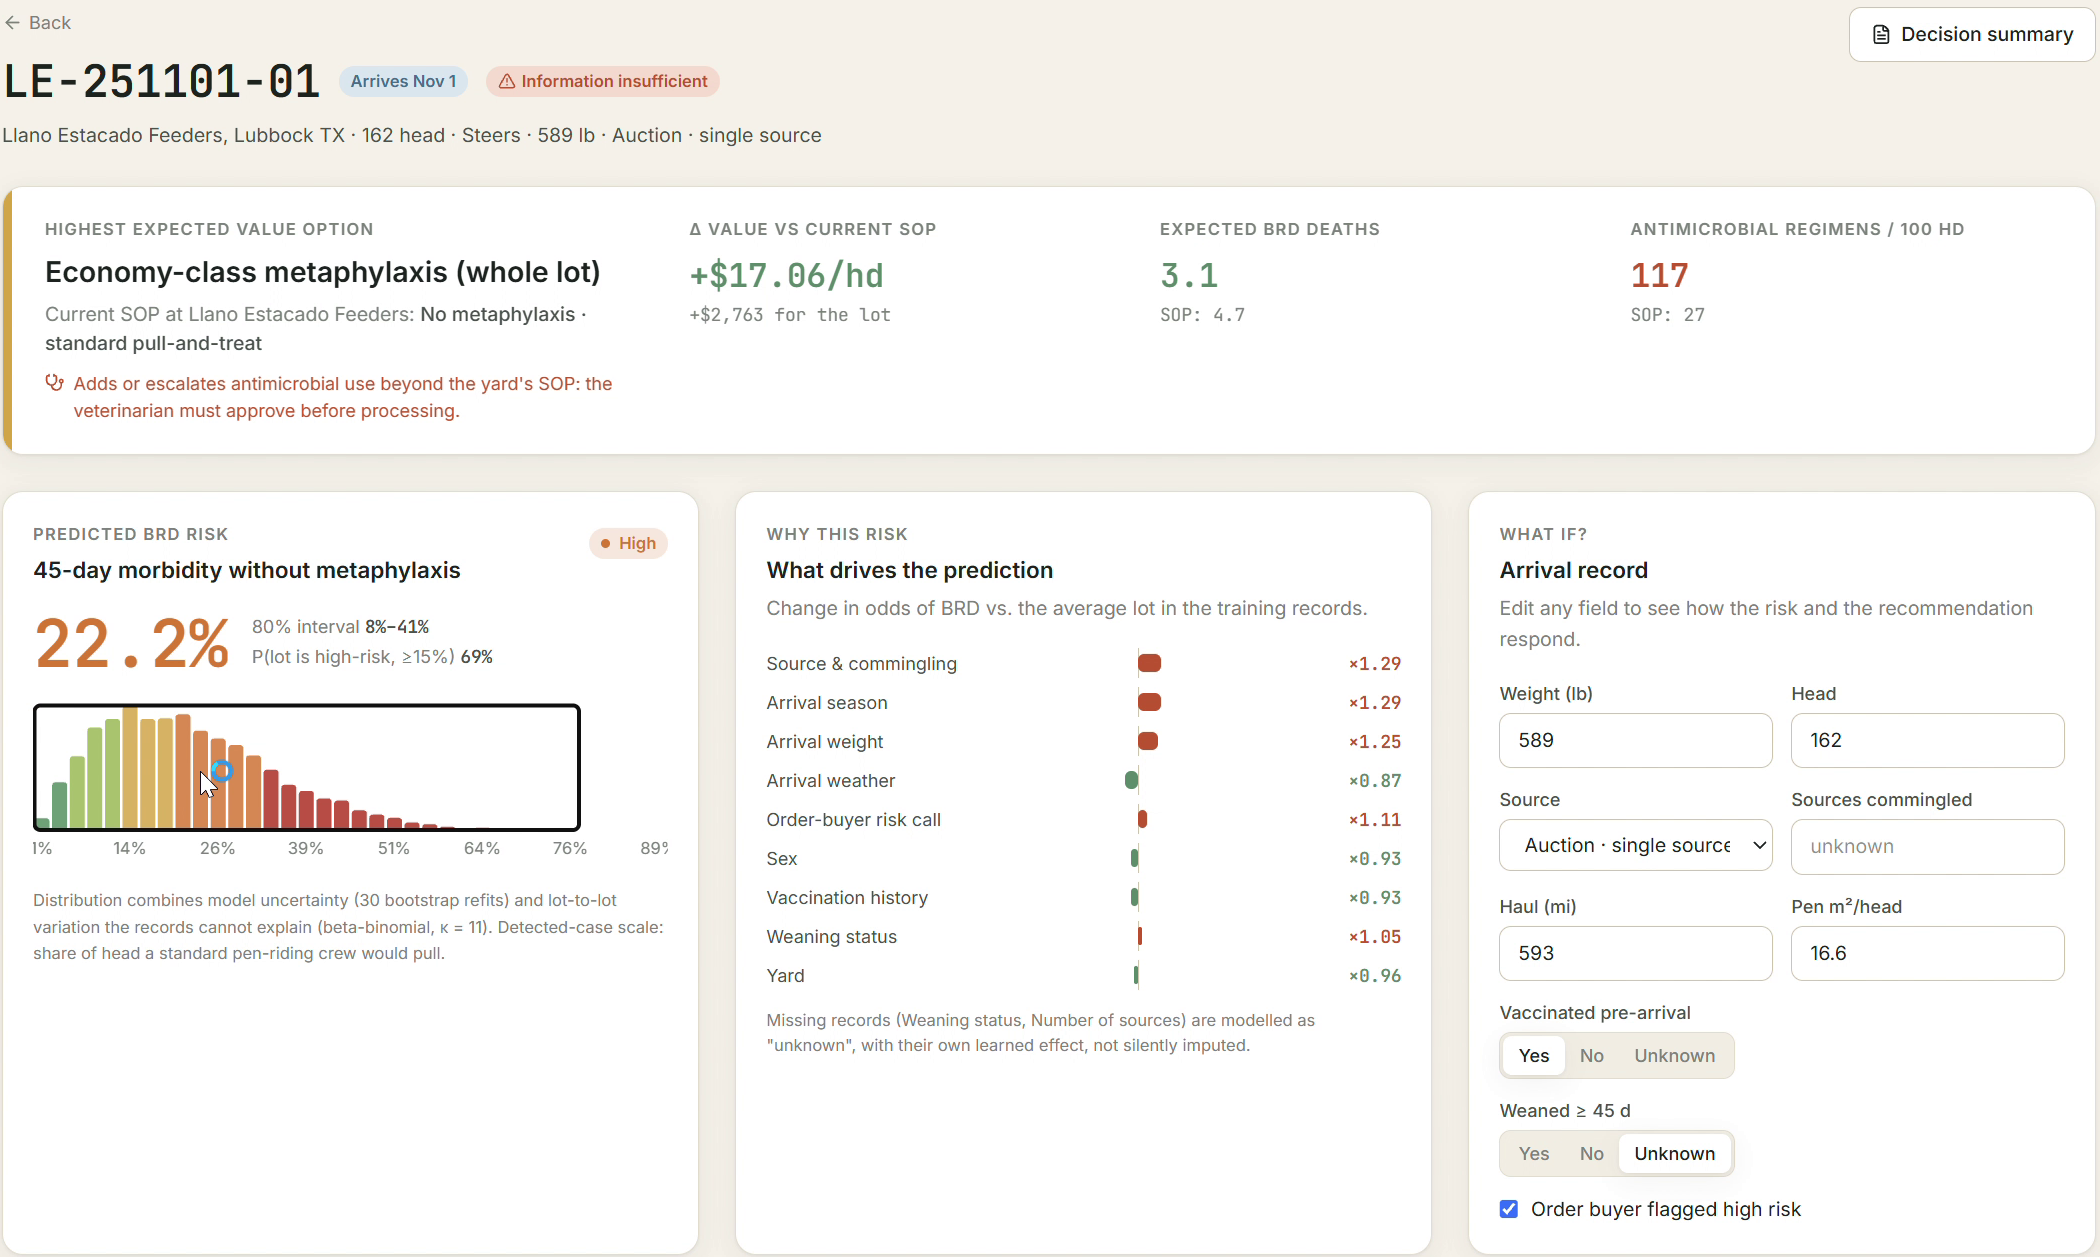
\includegraphics[width=\linewidth]{figures/lot_page.png}
  \caption{Lot page for LE-251101-01: the recommended option against the SOP, the risk distribution, the drivers of the prediction and the what-if panel used to test the missing weaning record.}
  \label{fig:lot}
\end{figure}

% =============================================================================
\section{Alternatives and projected consequences}

Per head over the feeding period, relative to the SOP. Value is feeding-period net return minus the \usd{3}/regimen stewardship weight; the dashboard states this basis under every value table.

\begin{table}[h]
\centering\small
\rowcolors{2}{rowshade}{white}
\begin{tabular}{@{}lccc@{}}
\toprule
\textbf{Option} & \textbf{$\Delta$ value vs SOP} & \textbf{Expected BRD deaths} & \textbf{Antimicrobial regimens} \\
\midrule
\textbf{Economy metaphylaxis} & \textbf{+\usd{17.06}} & 3.1 & 190 \\
Premium metaphylaxis + enhanced surveillance & +\usd{16.98} & 2.0 & 190 \\
Fever screen + enhanced surveillance & +\usd{16.82} & 2.7 & 81 \\
Premium metaphylaxis & +\usd{15.63} & 2.3 & 184 \\
Fever screen & +\usd{13.17} & 3.5 & 72 \\
No metaphylaxis, enhanced surveillance & +\usd{4.03} & 3.8 & 56 \\
No metaphylaxis, pull-and-treat (\textbf{SOP}) & --- & 4.7 & 43 \\
\bottomrule
\end{tabular}
\end{table}

Each option is simulated 400 times on the same paired futures; every page (lot list, lot page, demonstration, summary, model comparison) uses the same count, so they rank options identically. The top three options are within \usd{0.24}/head of each other, but they differ greatly in antimicrobial use: 190 regimens vs 81.

% =============================================================================
\section{Can the data support the decision?}

\begin{tcolorbox}[colback=warnbg,colframe=warn,boxrule=0.6pt,arc=2pt,left=6pt,right=6pt,top=4pt,bottom=4pt]
\textbf{\color{warn}Information insufficient.}
\begin{itemize}
  \item Knowing \textbf{weaning status} would change the recommendation with \textbf{100\pct} probability: either answer moves the decision away from economy metaphylaxis.
  \item Close call on antimicrobial use: economy metaphylaxis beats premium metaphylaxis with enhanced surveillance in only 60\pct{} of paired simulations, across a wide risk range (8--41\pct).
  \item The number of origins is also unknown and could change the recommendation (100\pct{} chance, worth $\approx$\,\usd{0.70}/head, below the \usd{1}/head ``need info'' threshold).
\end{itemize}
\end{tcolorbox}

\textbf{Weaning status} is the record that matters most. Learning it is worth $\approx$\,\textbf{\usd{208}} for the lot (\usd{1.29}/head):
\begin{itemize}
  \item if weaned $\rightarrow$ risk 16.5\pct: \textbf{fever screen + enhanced surveillance}, treating only feverish cattle (+\usd{9.15}/hd vs SOP, 63 regimens);
  \item if not weaned $\rightarrow$ risk 25.3\pct: \textbf{premium metaphylaxis + enhanced surveillance} for the whole lot (+\usd{23.29}/hd, 194 regimens).
\end{itemize}
So one phone call decides whether 162 head get a whole-lot antibiotic or only the feverish ones do. It is a stewardship decision as much as an economic one.

\begin{figure}[h]
  \centering
  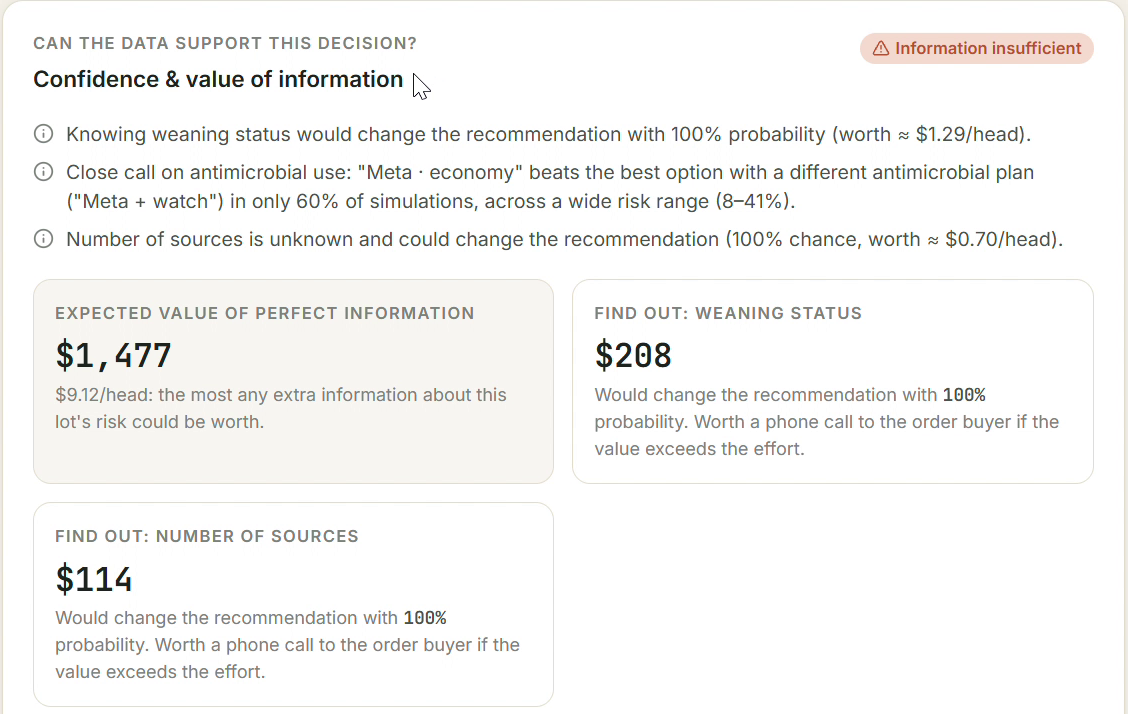
\includegraphics[width=0.72\linewidth]{figures/confidence_panel.png}
  \caption{Confidence and value-of-information panel for the lot: the reasons behind ``Information insufficient'', the expected value of perfect information, and what each missing record is worth.}
  \label{fig:conf}
\end{figure}

\lead{Model robustness} (lot page $\rightarrow$ ``Do the other risk models agree?''):
\begin{itemize}
  \item The two logistic models (22.2\pct) and the model average (20.0\pct) recommend economy metaphylaxis.
  \item The Rojas-predictor logistic, decision tree, random forest and boosted trees predict 17--21\pct{} and recommend the fever screen with enhanced surveillance (4 of 7).
  \item Every model agrees the SOP's ``pull and treat only'' is the wrong call (each model's own choice is +\usd{12.22} to +\usd{17.06}/hd better). They disagree only on how much antibiotic to use, exactly the question the phone call answers.
\end{itemize}

\textbf{Action:} call the order buyer about weaning before processing.

% =============================================================================
\section{Yard constraints}

The yard planner assigns economy metaphylaxis to this lot, the same as its stand-alone best option. Llano's capacity is not binding in this window: the hospital-pen peak is 82 of 170 places and both shadow prices are \usd{0}, so every lot can receive its own best option. (Capacity does bind at Palo Duro and Arkansas River, where pen-rider time is worth \usd{139} and \usd{1,377} per extra hour$\cdot$day.) Across all 39 Llano lots the plan is \textbf{+\usd{27.0}k} vs the SOP, with \textbf{56 vs 78} expected BRD deaths, at the cost of \textbf{1,888 vs 960} antimicrobial regimens.

Llano's SOP treats only lots under 550\,lb, so heavier but high-risk, buyer-flagged lots go untreated. Closing that gap is where the yard's gain comes from. Raising the stewardship weight on the planner traces how much of the extra antimicrobial use can be cut, and what each cut costs.

% =============================================================================
\section{Recommendation}

\begin{tcolorbox}[colback=boxbg,colframe=accent,boxrule=0.6pt,arc=2pt,left=6pt,right=6pt,top=4pt,bottom=4pt]
\textbf{Treat lot LE-251101-01 on arrival, with the intensity decided by one phone call.}
\begin{itemize}
  \item If the buyer confirms the calves were weaned $\geq$\,45 days, use a chute-side fever screen with enhanced surveillance: treat only febrile cattle.
  \item If they were not weaned, use premium metaphylaxis with enhanced surveillance.
  \item If the call can't be made before processing, use economy-class metaphylaxis (the best option on current records).
\end{itemize}
\end{tcolorbox}

Expected consequences of the default (economy metaphylaxis) vs SOP:
\begin{itemize}
  \item +\usd{17.06}/head after the stewardship weight (+\usd{2,763} for the lot);
  \item 3.1 vs 4.7 expected BRD deaths;
  \item 190 vs 43 antimicrobial regimens;
  \item peak hospital demand of 4.8 head from this lot.
\end{itemize}

% =============================================================================
\section{Veterinary review and record}

The option adds antimicrobial use beyond the yard's SOP, so it is marked \textbf{needs review} and queued for the veterinarian of record. The vet approves, modifies or declines it on the lot page (product, dose and withdrawal per label). \textbf{Decision Summary $\rightarrow$ Single lot $\rightarrow$ LE-251101-01} produces the signed one-page record (print/PDF, Markdown, JSON).

\vfill
{\footnotesize\color{gray} Records are synthetic, generated by a documented, seeded process calibrated to the supplied literature and driven by real NOAA weather. The case demonstrates the decision logic; it does not establish field performance. Medication-related outputs are decision support and require review by the veterinarian of record.}

\end{document}
